\subsection{Ecommerce websites vs news websites}
In our research, a crucial element was the comparison of two types of websites. This comparison enabled us, firstly, to hypothesize about the potential uses of cross-device tracking and, secondly, to understand when user data is more susceptible to being shared with third parties. We compared online shopping sites and news websites. This choice of categories was driven by the common use of cross-device tracking, which is typically needed either for advertising purposes, beneficial to sales-focused companies, or for targeting specific audiences, a tactic often employed by political entities. At the beginning of our study, we assumed that cross-device tracking would be more prevalent in online stores. However, the data we gathered did not confirm our assumptions. Instead, we were able to draw interesting conclusions about how these two types of sites collect and use sensitive user data, and what potential risks there might be for the users.

\subsubsection{Comparing Third-party requests}
\noindent 
\begin{minipage}{0.4\textwidth} 
    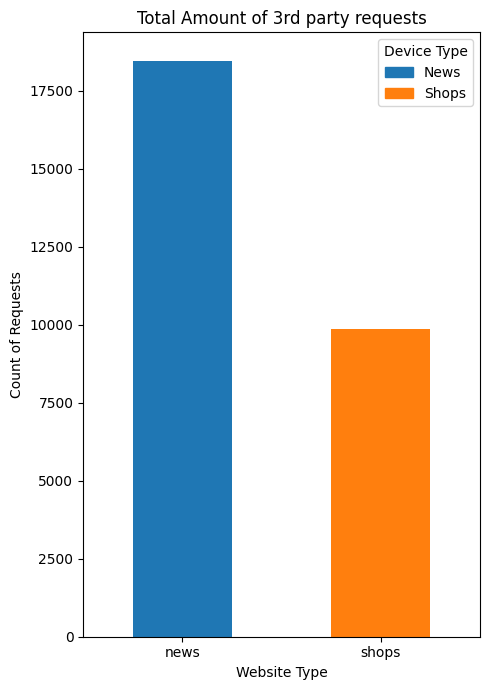
\includegraphics[width=\linewidth]{./assets/comparison1.png} 
\end{minipage}%
\hfill 
\begin{minipage}{0.5\textwidth} 
    One of the key aspects for comparison are third-party requests, as they are a primary indicator that sensitive data might be shared with third parties to create a more accurate user profile. We decided to find out which type of website makes more third-party requests. The chart demonstrates that in our dataset, news websites sent almost twice as many requests as online stores. This could be due to the fact that news websites almost always have more advertising, trackers for analytics, or social media widgets, which require reaching out to third-party servers. This makes such sites an ideal environment for cross-device tracking, and thus for collecting the maximum amount of user data.
\end{minipage}

\subsubsection{Comparing cookies set}
Cookies are a very important step in linking a user's activity on one device with their activity on another. Cookies also store information about the pages viewed, the time of site visits, and even the user's interaction scenario with the site, which are crucial for cross-device tracking. The presented chart shows that news websites set up five times more cookies than online stores. This is likely due to the fact that advertisers and website owners can not only personalize content but also the ads that are present on most news sites. Session synchronization allows determining the type of content that the user views on each device, which is especially important for news sites, as users often read the news both on mobile devices while away from home and on computers at home. In addition to the previously listed impacts of cross-device tracking on ad targeting, such results also raise the issue that users might end up in a sort of news bubble, as algorithms, using the collected data, offer them more similar content with which the user actively interacts, thus always receiving similar content.

\noindent 
\begin{minipage}{0.6    \textwidth} 
    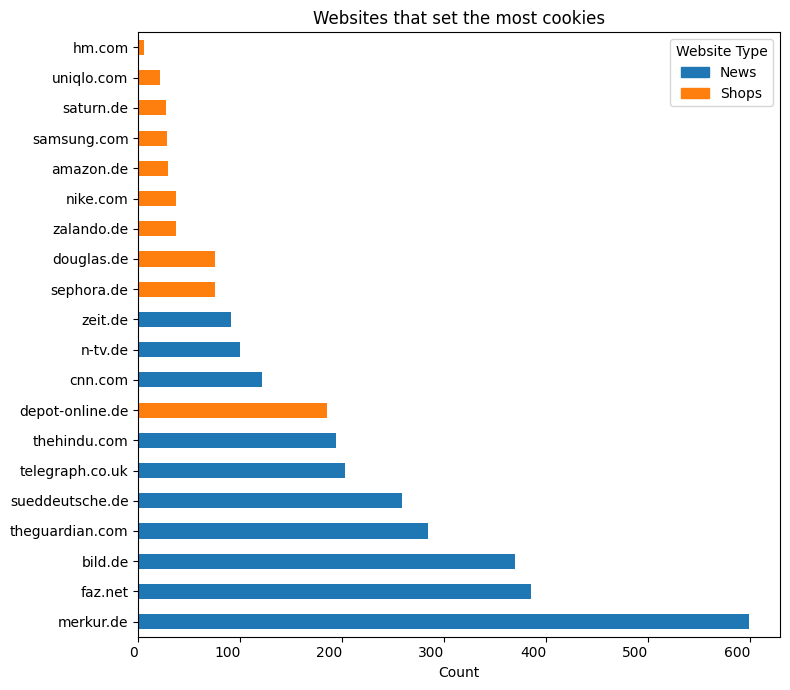
\includegraphics[width=\linewidth]{./assets/comparison21.png}
\end{minipage}
\hfill 
\begin{minipage}{0.35\textwidth}
    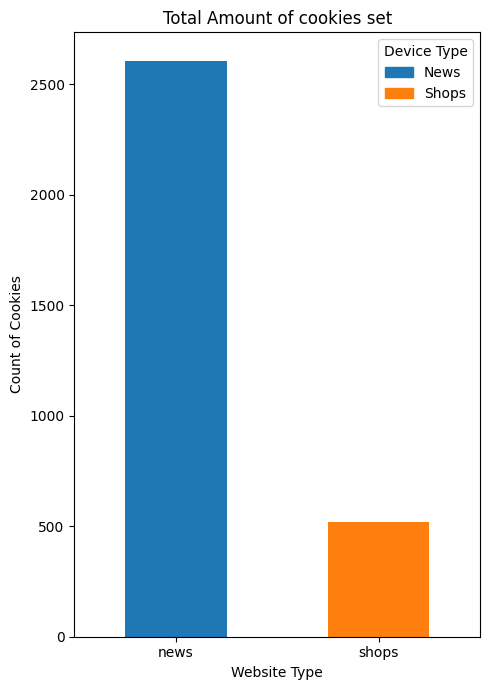
\includegraphics[width=\linewidth]{./assets/comparison2.png}
\end{minipage}

\subsubsection{Shared email addresses}
\noindent 
\begin{minipage}{0.4\textwidth} 
    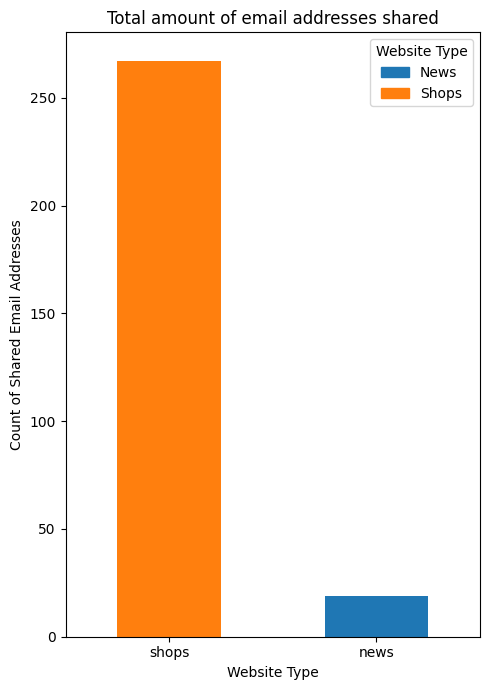
\includegraphics[width=\linewidth]{./assets/comparison3.png} 
\end{minipage}
\hfill 
\begin{minipage}{0.5\textwidth} 
    One of the most interesting findings of our research is the fact that online stores distributed email addresses more than ten times as often as news websites. The email address is a key identifier for linking a user's various devices. Therefore, it can be concluded that online stores also use cross-device tracking to create a unified customer profile, but apparently employ methods different from those used by news platforms. As noted earlier, the company Sephora initiated a significant portion of the email address transfers, raising concerns about the privacy of data used by this company. In any case, such research results could be due to the fact that sales-oriented websites are more interested in retaining customers by offering personalized discounts and deals via email, while for news sites, individual user interaction is not as crucial as content and advertising targeting.
\end{minipage}

\subsection{Mobile vs desktop}
We compared mobile and desktop devices in terms of the total amounts of each analysis category.
\begin{figure}[h!]
    \centering
    
    \begin{subfigure}[b]{0.28\textwidth}
        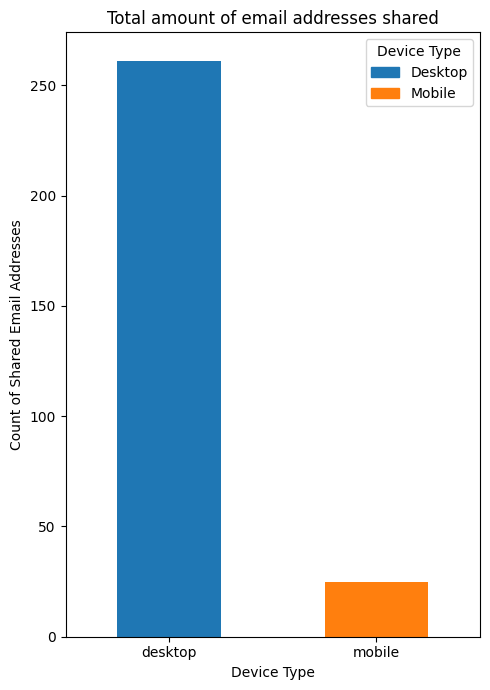
\includegraphics[width=\textwidth]{./assets/comparison4.png}
        \caption{}
        \label{fig:3rdparty}
    \end{subfigure}
    \hfill
    \begin{subfigure}[b]{0.28\textwidth}
        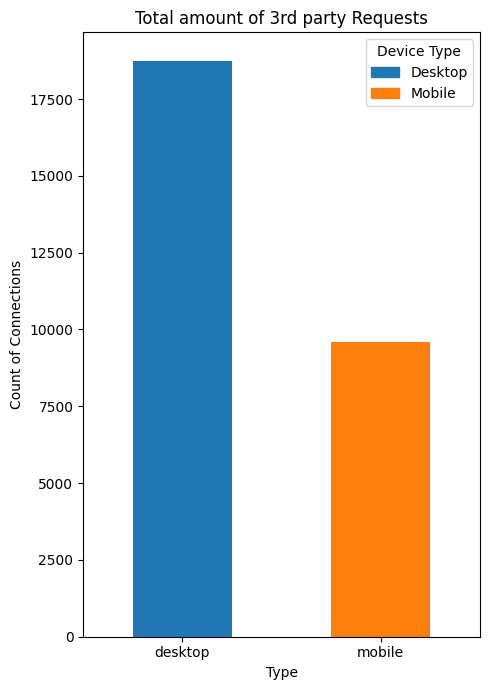
\includegraphics[width=\textwidth]{./assets/comparison5.png}
        \caption{}
        \label{fig:cookies}
    \end{subfigure}
    \hfill 
    \begin{subfigure}[b]{0.28\textwidth}
        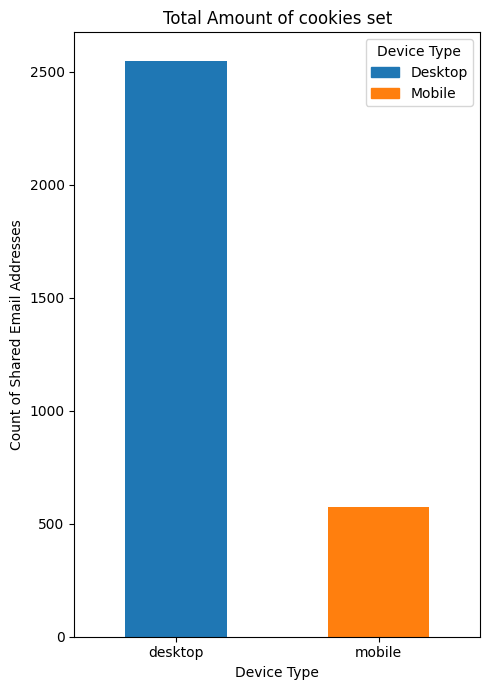
\includegraphics[width=\textwidth]{./assets/comparison6.png}
        \caption{}
        \label{fig:emails}
    \end{subfigure}
    
    \label{fig:trackingmetrics}
\end{figure}